\documentclass[a4paper]{article}
\usepackage[utf8]{inputenc}
% \usepackage[UTF8]{ctex}
\usepackage{amsmath, amsthm, amssymb, calrsfs, wasysym, verbatim, bbm, color, graphics, geometry}
\usepackage{graphicx}
\usepackage{url}
\usepackage{esvect}
\usepackage{mathtools}
\usepackage{bm}
\usepackage{latexsym}
\usepackage{mathrsfs}
\usepackage{amsfonts}
\usepackage{enumitem}
\usepackage{xcolor, color, textcomp}
\usepackage{textcomp}
\usepackage{float}
\usepackage{nccmath}

\usepackage{dirtree}
\usepackage{hyperref}
\usepackage{caption}

\usepackage{listings}

\definecolor{codegreen}{rgb}{0,0.6,0}
\definecolor{codegray}{rgb}{0.5,0.5,0.5}
\definecolor{codepurple}{HTML}{C42043}
\definecolor{backcolour}{HTML}{F2F2F2}
\definecolor{bookColor}{cmyk}{0,0,0,0.90}
\color{bookColor}

\lstdefinestyle{mystyle}{
    backgroundcolor=\color{backcolour},
    commentstyle=\color{blue},
    keywordstyle=\color{codepurple},
    numberstyle=\numberstyle,
    basicstyle=\footnotesize\ttfamily,
    breakatwhitespace=false,
    breaklines=true,
    captionpos=b,
    keepspaces=true,
    numbers=none,
    showspaces=false,
    showstringspaces=false,
    showtabs=false,
    morekeywords={pip, install, bokeh}
}
\lstset{style=mystyle}

\newcommand\numberstyle[1]{%
    \footnotesize
    \color{codegray}%
    \ttfamily
    \ifnum#1<10 0\fi#1 |%
}

% Default fixed font does not support bold face
\DeclareFixedFont{\ttb}{T1}{txtt}{bx}{n}{12} % for bold
\DeclareFixedFont{\ttm}{T1}{txtt}{m}{n}{12}  % for normal

% Custom colors
\definecolor{deepblue}{rgb}{0,0,0.5}
\definecolor{deepred}{rgb}{0.6,0,0}
\definecolor{deepgreen}{rgb}{0,0.5,0}

\newenvironment{faq}{\begin{description}[style=nextline]}{\end{description}}

\title{\textbf{Enhanced Movie Database:\\ Reviews, Searching, Rating the Movies}}
\author{Liu Yihan (1170100177), Cai Haoming (117010002), Huang Zihao (117010103), \\Chen Haoyu (117010013), Cao Yuji (117010007)}

\begin{document}

\date{}
\maketitle

\begin{abstract}
In decades, people fuel the online informalized data with vast streams of review and rating on various movie community websites. Therefore, the existence of those abundant data can not be ignored by any film archives which engage in the research of movies' overview. However, as a well-known movie community website providing plenty of useful movie information, Douban movie database is not able to serve as an effective source for aggregating movie reviews and research due to its limited data search and analysis methods. To address these problems effectively, an enhanced database is proposed for reviewing, searching, analyzing and rating movies in this report. In this database, to facilitate data searching and analysis, lossless decomposition is necessary. Therefore, it is designed in second normalized form and third normalized form. In addition, it provides adequate SQL queries that are used for more comprehensive analysis and data mining about movies. By applying this design, the film archives are able to do more specific operations and examine the data more extensively for their research.

\end{abstract}
% \section{Abstract}
\section{Background and Motivation}
\paragraph{Background}Movies are highly popular on the Web. There are several web resources dedicated to movies and many others containing movie-related information. For the two famous movie database website Douban and IMDb, the Internet Movie Database (IMDb) claims to be "the world's most popular and authoritative source for movie, TV and celebrity content," offering a searchable database which includes more than two million films, television, and entertainment programs and attracting more than 150 million unique monthly visitors (IMDb, 2013). At the same time,9 Douban Movie ranks No.1 in the iOS App Store in 2012 with about 200 million registered users as of 2013 \cite{Alexa}. With such a large number of users, these movie databases attract lots of attention to the movie analysis study and research, which engages in movie reviews and ratings. For instance, Jie Yang and Brian Yecies designed an innovative collection and analytic tool, termed Douban-Learning, which is a big-data framework for analyzing Douban movie reviews \cite{yang2016mining} and Sandra Carvalho designed an emotional movie database (EMDB) based on IMDB data \cite{carvalho2012emotional}.
\paragraph{Motivation}However, most movie database websites are only designed for registered members' rating and writing reviews, while both the EMDB and Douban-Learning needs to preprocess first to get the origin movie data and then for analysis use. Besides, the Web-only has limited search methods for basic information and poor analysis methods for top-rated movies. For researchers, such data can not be used directly and efficiently, and the scattered movie data still need to be aggregated for use. Hence, we designed an enhanced movie database for reviewing, searching, analyzing, and rating movies, especially for researchers.
  \section{Method}
  The report contains four phases:
  \begin{itemize}
    \item Movie data pre-processing: web crawler is applied in this part to get the origin movie data from the official web and Douban movie, and more than 90000 movies webpage are fetched.
    \item Database Design: design the backend database structure of the enhanced movie database, containing E-R diagram design and schema design which conforms to BCNF\@.
    \item Database implementation: process the data and split them into several tables for import to the database directly. Besides, this part also contains the website visualization and database querying design under the website.
    \item Analysis: the preliminary analysis based on the website visualization and the movie data, including the annual trend of rating, box office, counting, etc.
  \end{itemize}

\section{Data Collection}
  \subsection{Web Crawler}
  The web crawler is a method that automatically simulates a human's browse using programs. No matter what kind of data it is, as long as it exists on a webpage, it can be fetched by the crawler program. Therefore, web crawlers are suitable for fetching massive and open-source information on a website in a short time.
  \subsection{Inconstant IP}
  Their tools contain checking IP addresses, browser's user-agent, request headers, etc. Among them, blocking IP addresses is the most common and efficient way to obstruct vicious requests. Douban uses this strategy, as well. Therefore, how to overpass this protection is one of the core parts of our program. \par
  We could decrease the frequency of access to avoid websites to block our IP, but it would waste too much time. It seems that using an inconstant IP address is the only method we could choose. In our project, we bought available IP addresses from a proxy. With the help of inconstant IP addresses, we could fetch lots of data without being clocked. We use more than 40 thousand IP addresses to obtain almost 300 thousand items, such as actors, awards, and movies.


  \begin{figure}[H]
    \centering
    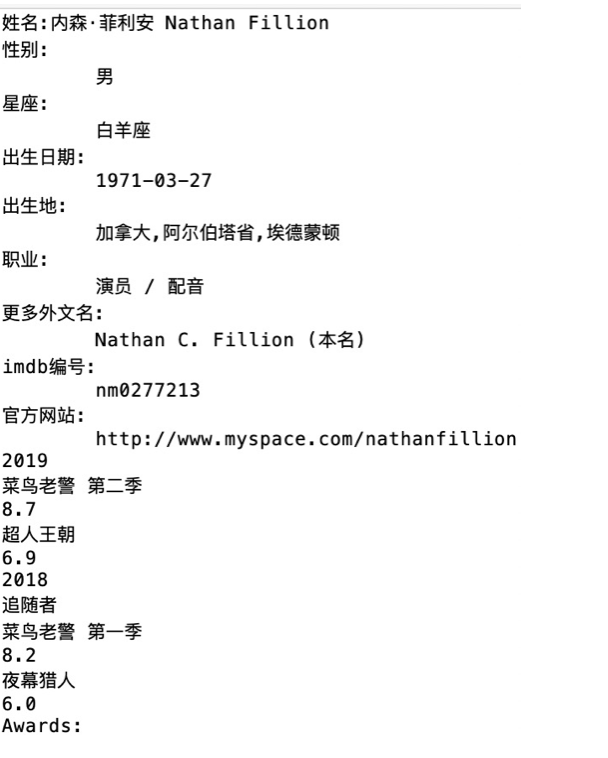
\includegraphics[width=200pt]{figures/raw_data.png}
    \caption{Raw data}
    \label{fig:raw}
  \end{figure}
  \subsection{Data Fetching}
Libraries used to fetch web elements are various. Here we use an elegant library named Beautiful Soup. Calling ‘find’ in Beautiful Soup, the precise search could be implemented. Those massive raw files are required to further process to form the initial version of CSV files. We show this process in Figure~\ref{fig:raw} and Figure~\ref{fig:initial_process}.
  \begin{figure}[H]
    \centering
    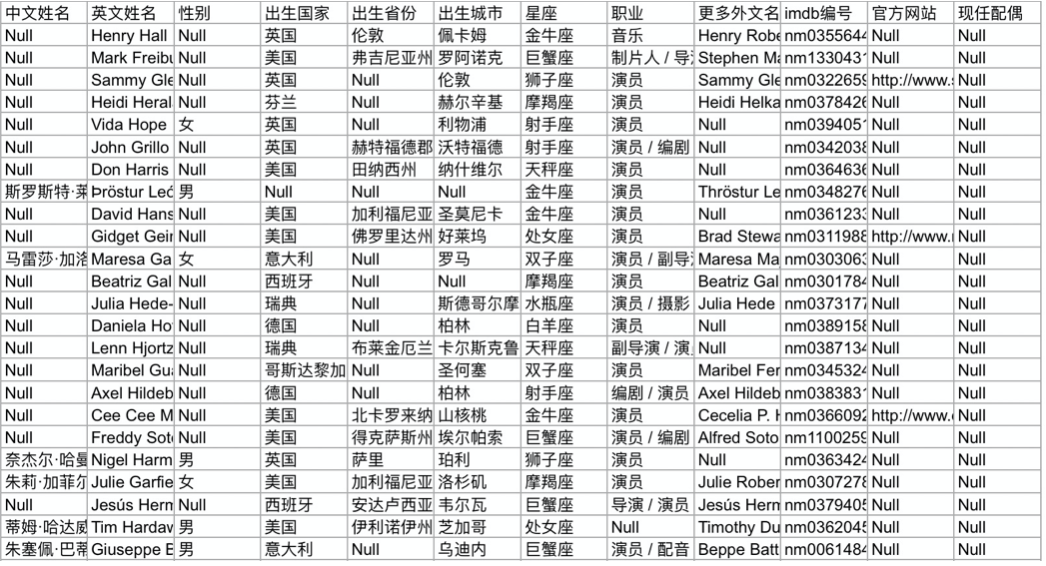
\includegraphics[width=300pt]{figures/processed_data.png}
    \caption{Initial version of processed data}
    \label{fig:initial_process}
  \end{figure}

\section{Database Design}
After we have all the data we need, we can start to design our database. We need to find a way that can store all the useful data in a structural way. The design needs two major steps. The first step is the E-R diagram design and the latter one is schema design.
  \subsection{E-R Diagram Design}
As mentioned before, we got the data from different sources. In other words, they don't have a uniform data structure of a consistent data label. So, we decided to use a data-oriented way to design our database. Based on the data we had, we abstracted all the entities and attributes. We have several versions of the E-R diagram. The one shown in Figure \ref{fig:er} below is our final version. \par
  \begin{figure}[ht]
    \centering
    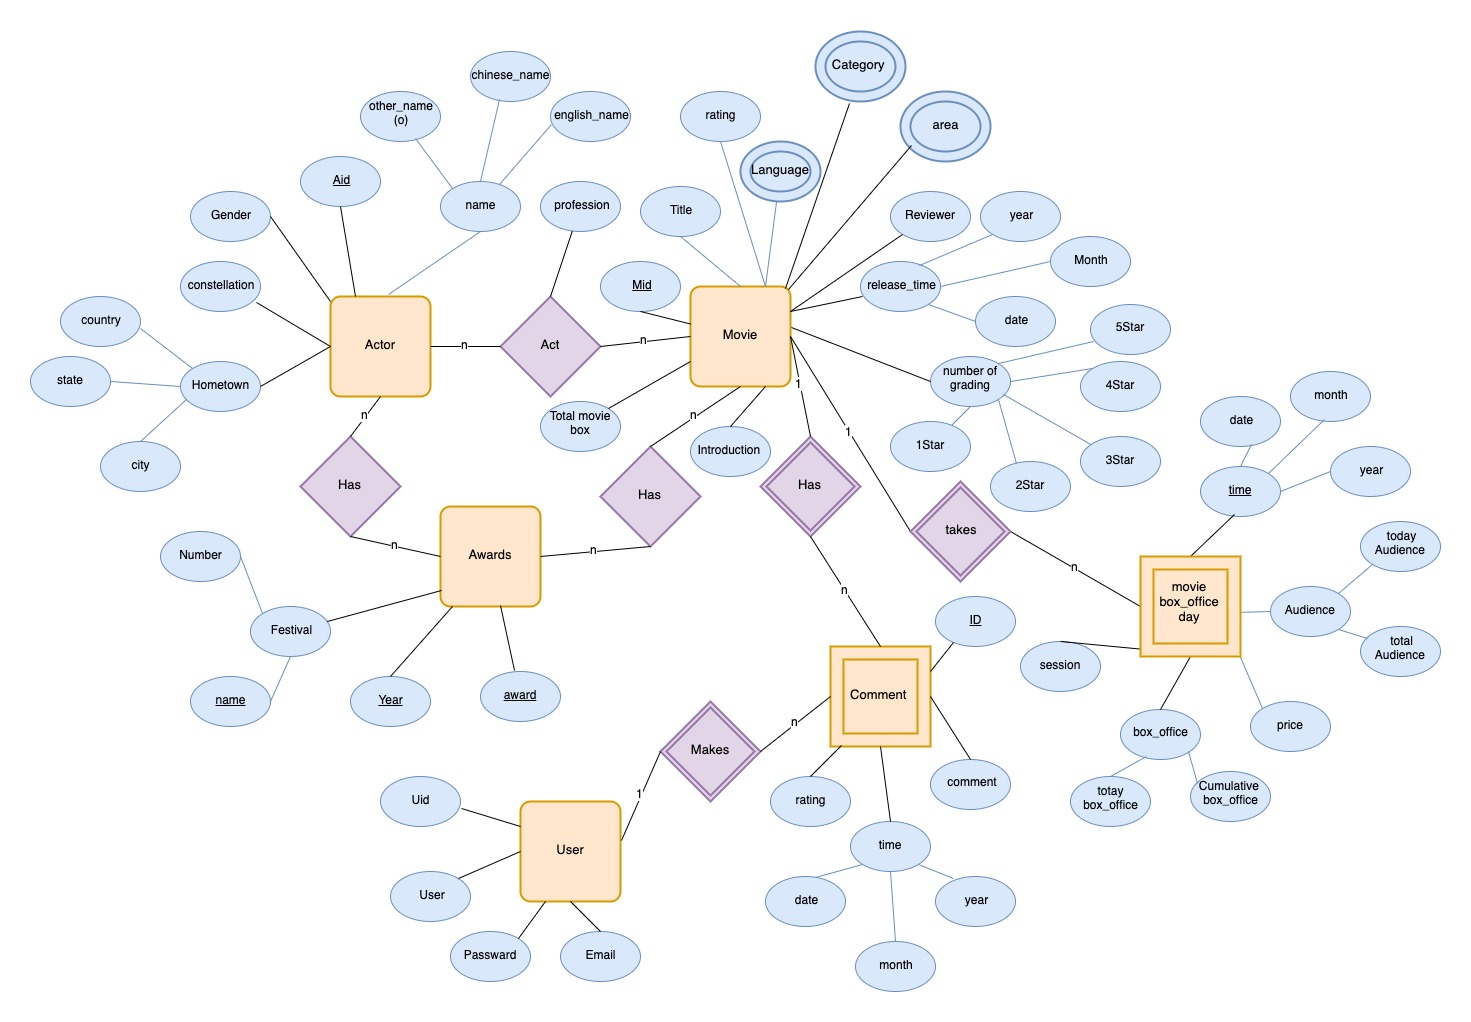
\includegraphics[width=\textwidth]{figures/er.jpeg}
    \caption{E-R diagram}
    \label{fig:er}
  \end{figure}
There are six basic entities in our design. They are Movie, User, Comment, the Movie Box Office of each day, Awards and Actor. In these six entities, comment and movie box office of each day are weak entities. The comment depends on the user and a specific movie, and the movie box office of each day depends on a specific movie. Each of the six entities has some relationships connected with others. The relationships are described below:
    \begin{itemize}
      \item An actor can win several awards and an award can give to many actors that's an N to N relationship.
      \item A movie can also earn many awards and an award can also be given to many movies, which is also an N to N relationship.
      \item An actor can perform in many movies and a movie can also have many actors.
      \item A movie can have multiple Movie Box Offices of different days but a specific movie box office of one day only refers to a specific movie.
      \item Each movie can have multiple comments, but a specific comment can only be made to a specific movie.
      \item Each user can make several comments, but a specific comment can only be owned by a specific user.
    \end{itemize}
For each of the six entities, it has its own attributes which are listed in the diagram.
  \subsection{Schema Design}

  \begin{figure}[H]
    \centering
    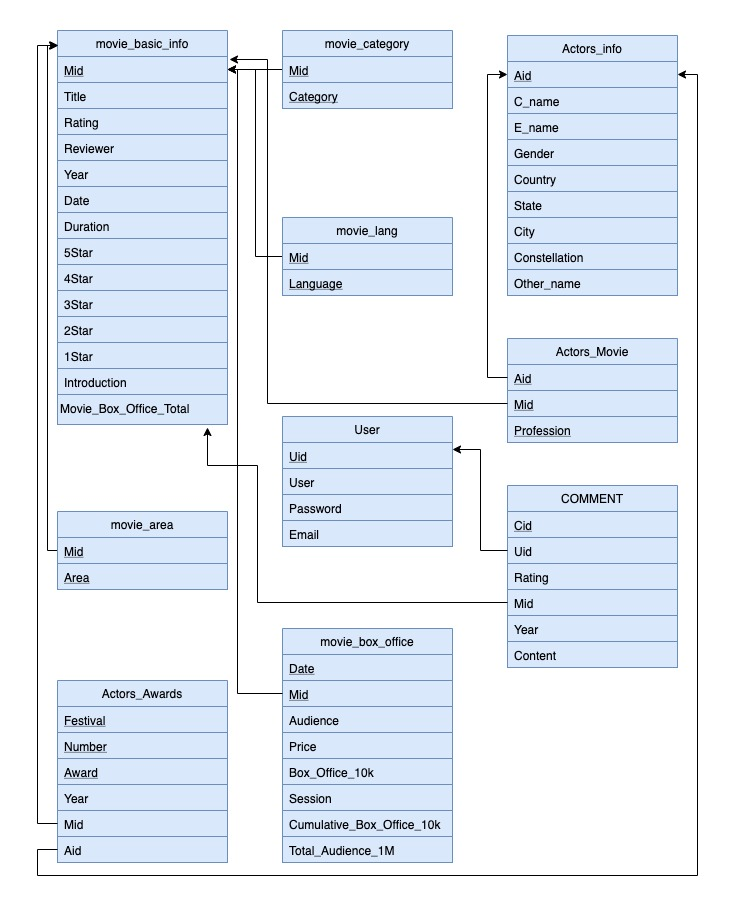
\includegraphics[width=300pt]{figures/schema.jpg}
    \caption{Schema Of the Database}
    \label{fig:schema}
  \end{figure}

Based on the E-R diagram shown above, our schema design is created. The Figure~\ref{fig:schema} shown below is our last version. \par

The last version of the schema satisfies the BCNF\@. To design the schema, we first make each entity in the E-R diagram to be a table, then decompose them into smaller tables, until each of them satisfies the BCNF\@. There is something special in the design: the table movie area, movie category and movie language only have two attributes that is because they are multivalued attributes of the movie entity. They have an N to N relationship to movies. To reduce the information redundancy, we make these 3 attributes to have their table. The FDs for each of the table are list below:
\begin{itemize}
  \item movie\_basic\_info:
    \begin{fleqn}
      \begin{align*}
      Mid \rightarrow &Title, Rating, Reviewer, Year, Date, Duration, 5Star, 4Star, 3Star, 2Star, 1Star, \\
      &introduction, Movie\_Box\_Office\_Total
      \end{align*}
    \end{fleqn}

  \item Actor\_Awards
        \begin{fleqn}
          \begin{align*}
      &Festival, Number, Award \rightarrow Year, Mid, Aid \\
      &Festival, Year, Award \rightarrow Number, Mid, Aid
          \end{align*}
        \end{fleqn}
  \item User:
        \begin{fleqn}
          \begin{align*}
     &Uid \rightarrow User, Password, Email
          \end{align*}
        \end{fleqn}
  \item movie\_box\_office:
        \begin{fleqn}
          \begin{align*}
       Date, Mid \rightarrow &Audiences, Price, Box\_Office\_10k, Session, \\ &Cumulative\_Box\_Office\_10k, Total\_Audience\_1M
          \end{align*}
        \end{fleqn}
  \item Actor\_info:
    \begin{fleqn}
      \begin{align*}
      Aid \rightarrow C\_name, E\_name, Gender, Country, State, City, Constellation, Other\_name
      \end{align*}
    \end{fleqn}
  \item COMMENT:
    \begin{fleqn}
      \begin{align*}
       Cid \rightarrow Uid, Rating, Mid, Year, Content
      \end{align*}
    \end{fleqn}
\end{itemize}

\section{Database Implementation}
\subsection{Data Processing}
As mentioned above, we gather the data from Douban Website and other professional websites using web crawlers. It consists of movies' information, reviews' information, actors' information, and information about movie awards like Oscar. Moreover, the data could be dirty because of inaccurate, incomplete, or inconsistent input. After data collection, despite reallocating according to the schema of our database for the convenience of importing data to our database, we still need data cleansing to rewrite the data easily. \par
We implemented data cleaning first, which detected and removed corrupt or inaccurate records from the database and then modified the dirty data. For instance, the unit of the movie box did not conform to any format in MySQL. Therefore, we invoked eval\(\) function in python to replace the origin string format into an integer. After data cleaning, since the data were fetched from multiple datasets, we implemented data matching and data reorganization to combine data from different data sets and fulfill our requirements, which could be considered as a lossless decomposition of the original data with the Mid(Movie ID) attribute as the super key. As for linking the same movie from different data sets, we performed record matching based on their titles and the corresponding release years.

\subsection{Web Visualization}
In order to provide a better way to demonstrate our database, a web-based front end application is implemented using Bokeh and Sqlite3 Library in Python. Bokeh is an interactive visualization library and Sqlite3 is a C-language library that implements a SQL database engine. In the application, the Bokeh library helps to demonstrate and visualize the data using various methods like data tables and diagrams. The Sqlite3 library contributes to process SQL queries in the database engine and extracts corresponding data. The commands to run this application is listed in Appendices Listing~\ref{lst:web}. To demonstrate our database, we implement this front end application, which consists of two Tabs: data table and iterative explorer diagram. \par

\subsubsection{Data Table Tab}
Data Table Tab extracts the data from the Movie database and demonstrates it according to the SQL query in the textInput widget. When a user inputs a SQL query and presses ENTER key, the SQL query is passed to the Bokeh server and being executed by the Sqlite3 engine to select the data. Then the data is returned back to the Bokeh serve, rendered by the Bokeh server and displayed on the web browser.

\begin{figure}[H]
  \centering
  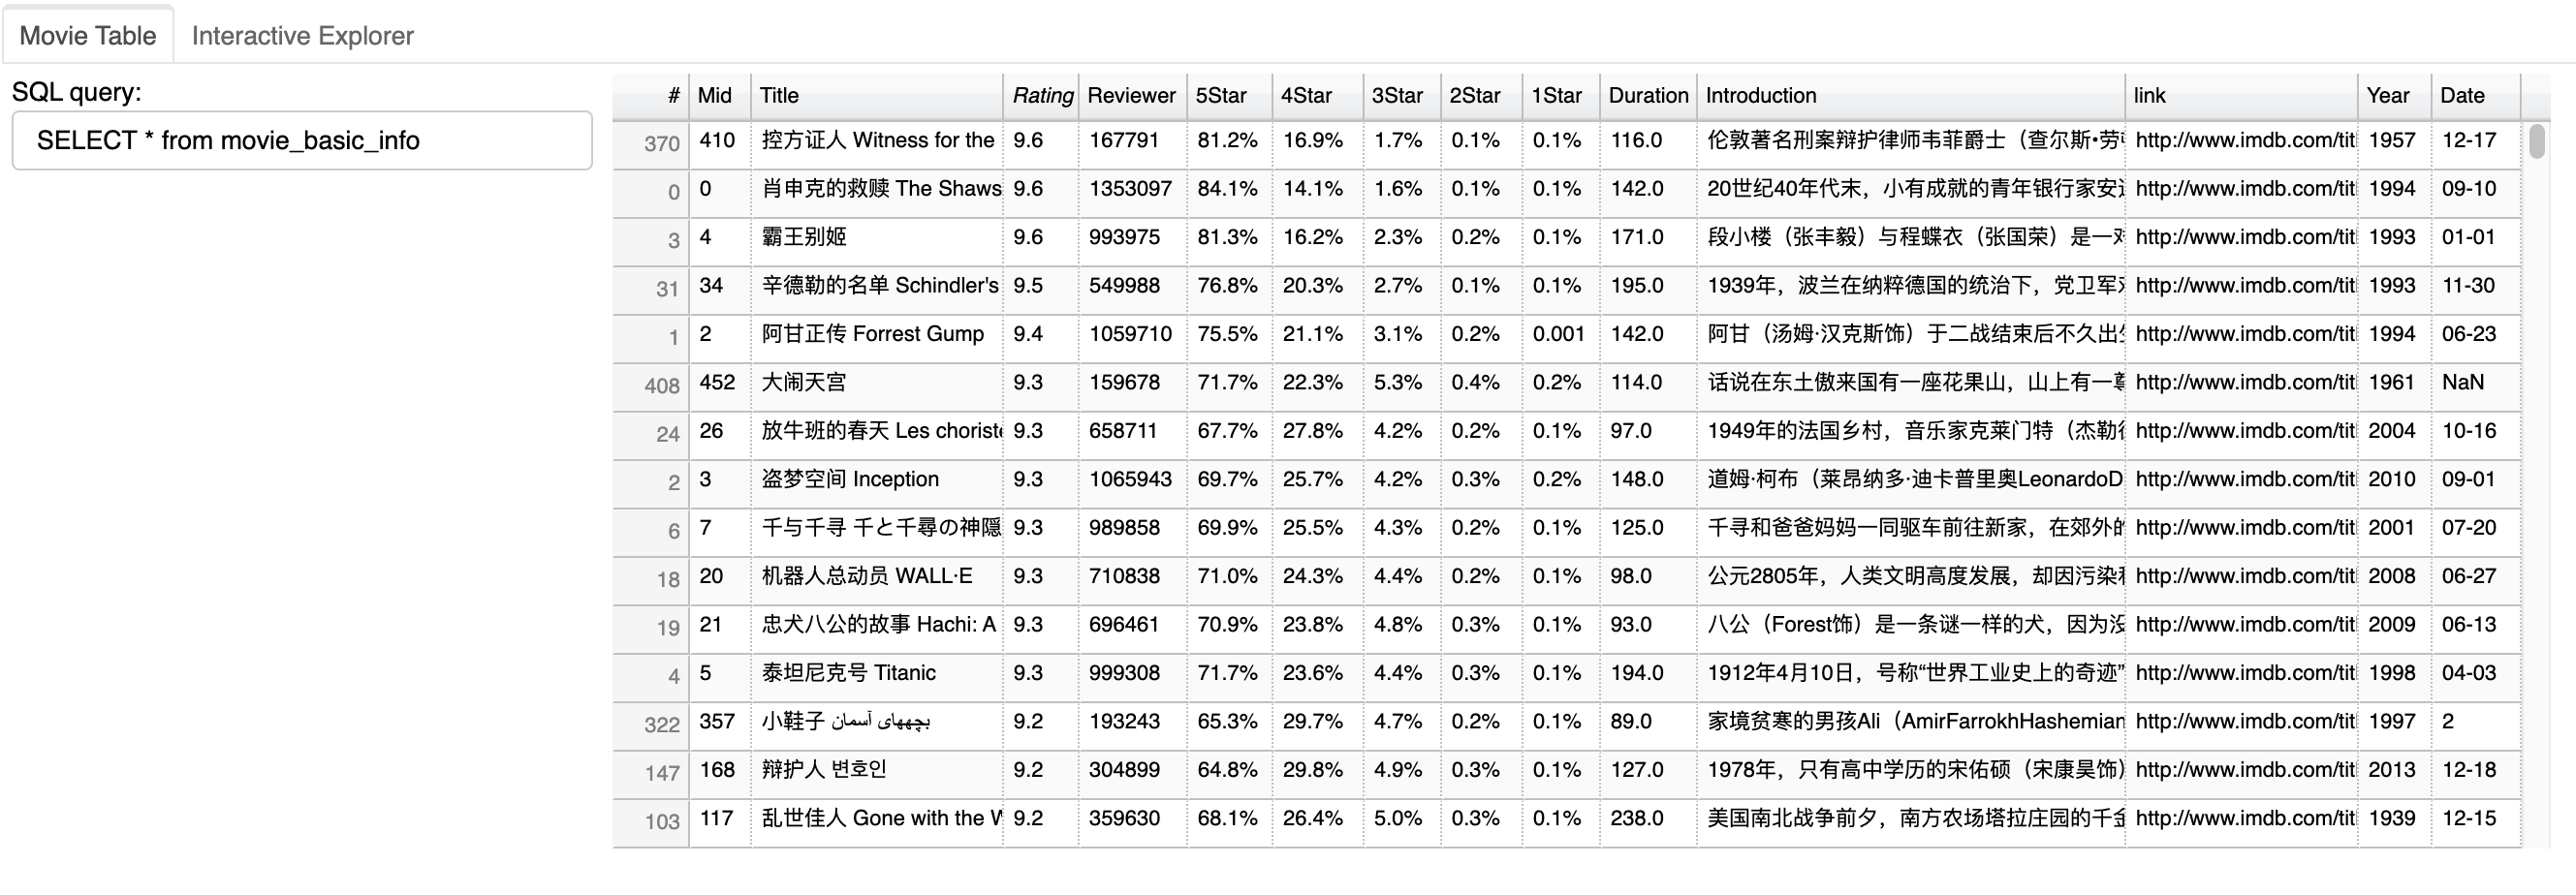
\includegraphics[width=\textwidth]{figures/data_table.png}
  \label{fig:datatable}
  \caption{Data table tab in web visualization}
\end{figure}

% FIXME add process diagram
\subsubsection{Iterative Explorer Diagram}
\begin{figure}[H]
  \centering
  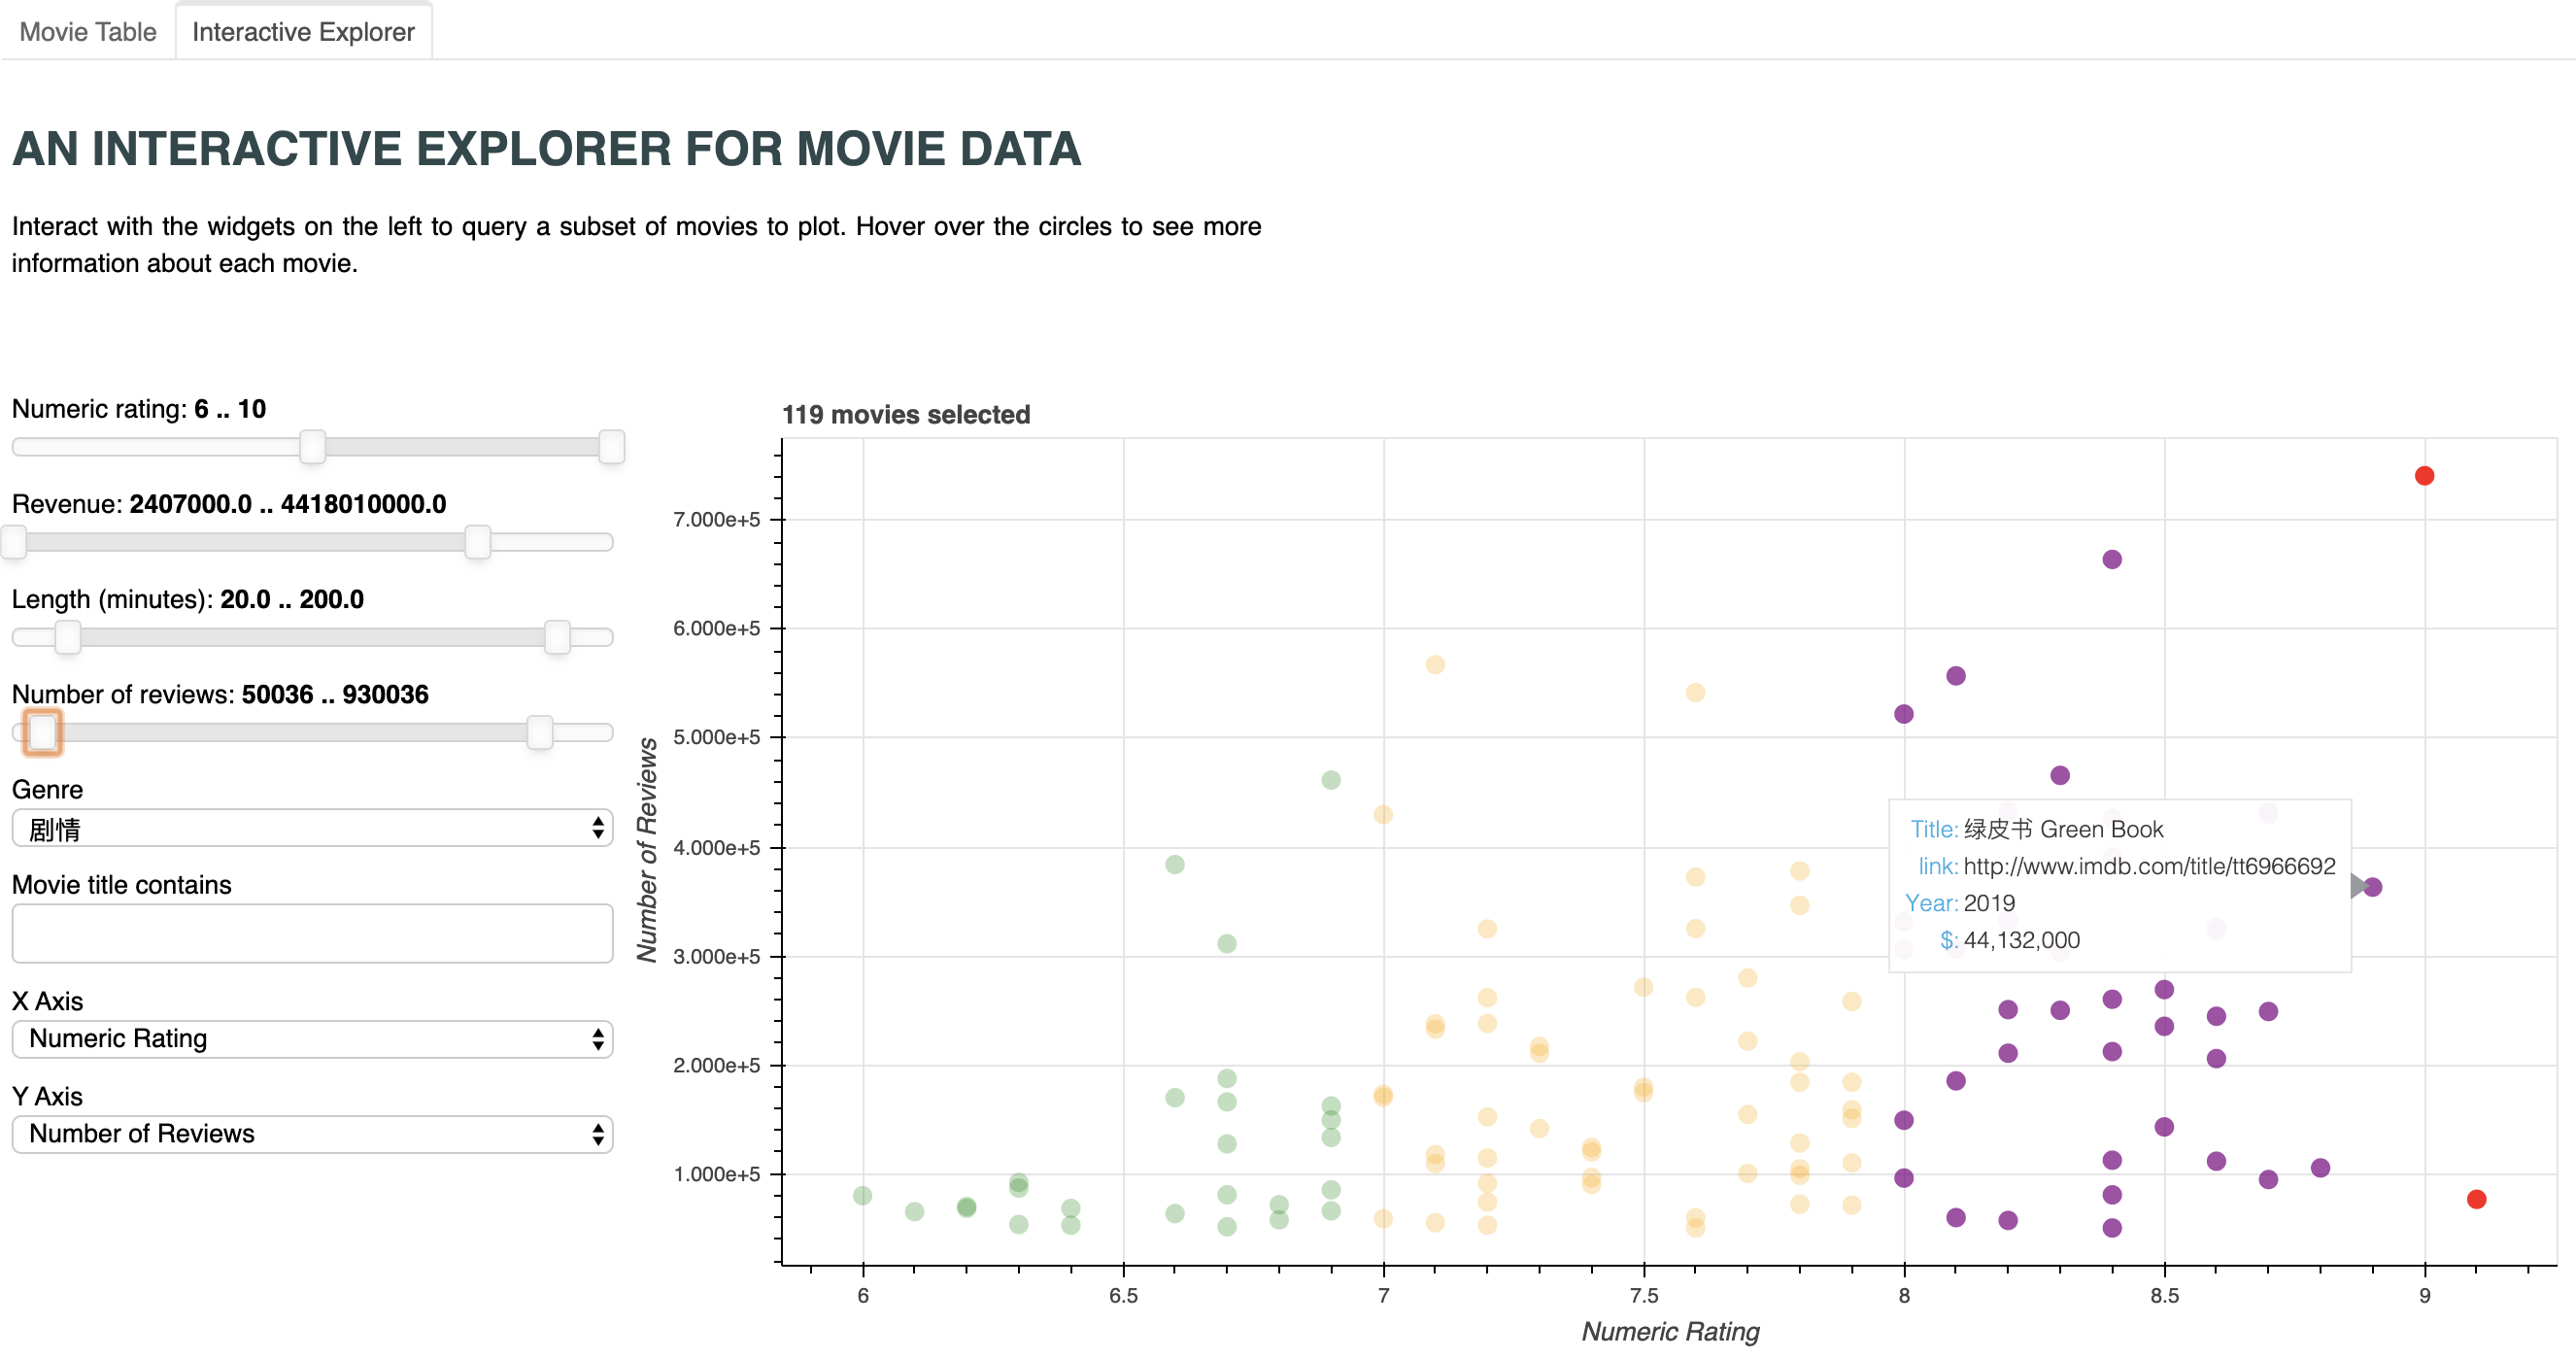
\includegraphics[width=\textwidth*4/5]{figures/explorer.png}
  \caption{Iterative explorer tab in web visualization}
  \label{fig:iterative_explorer}
\end{figure}
Iterative Explorer Diagram demonstrates the movies with a circle diagram where each movie is represented by a circle in the diagram and the darker the color, and higher rating the movie is. By selecting various criteria in the left column, the Bokeh will automatically compose these different constraints and instruct the Sqlite3 database to extract the corresponding data and visualize them on the diagram. In addition, a user is able to select different attributes on the X and Y axis to explore the different relationships between rating, length of movies, revenue and so forth.

\begin{figure}[H]
  \centering
  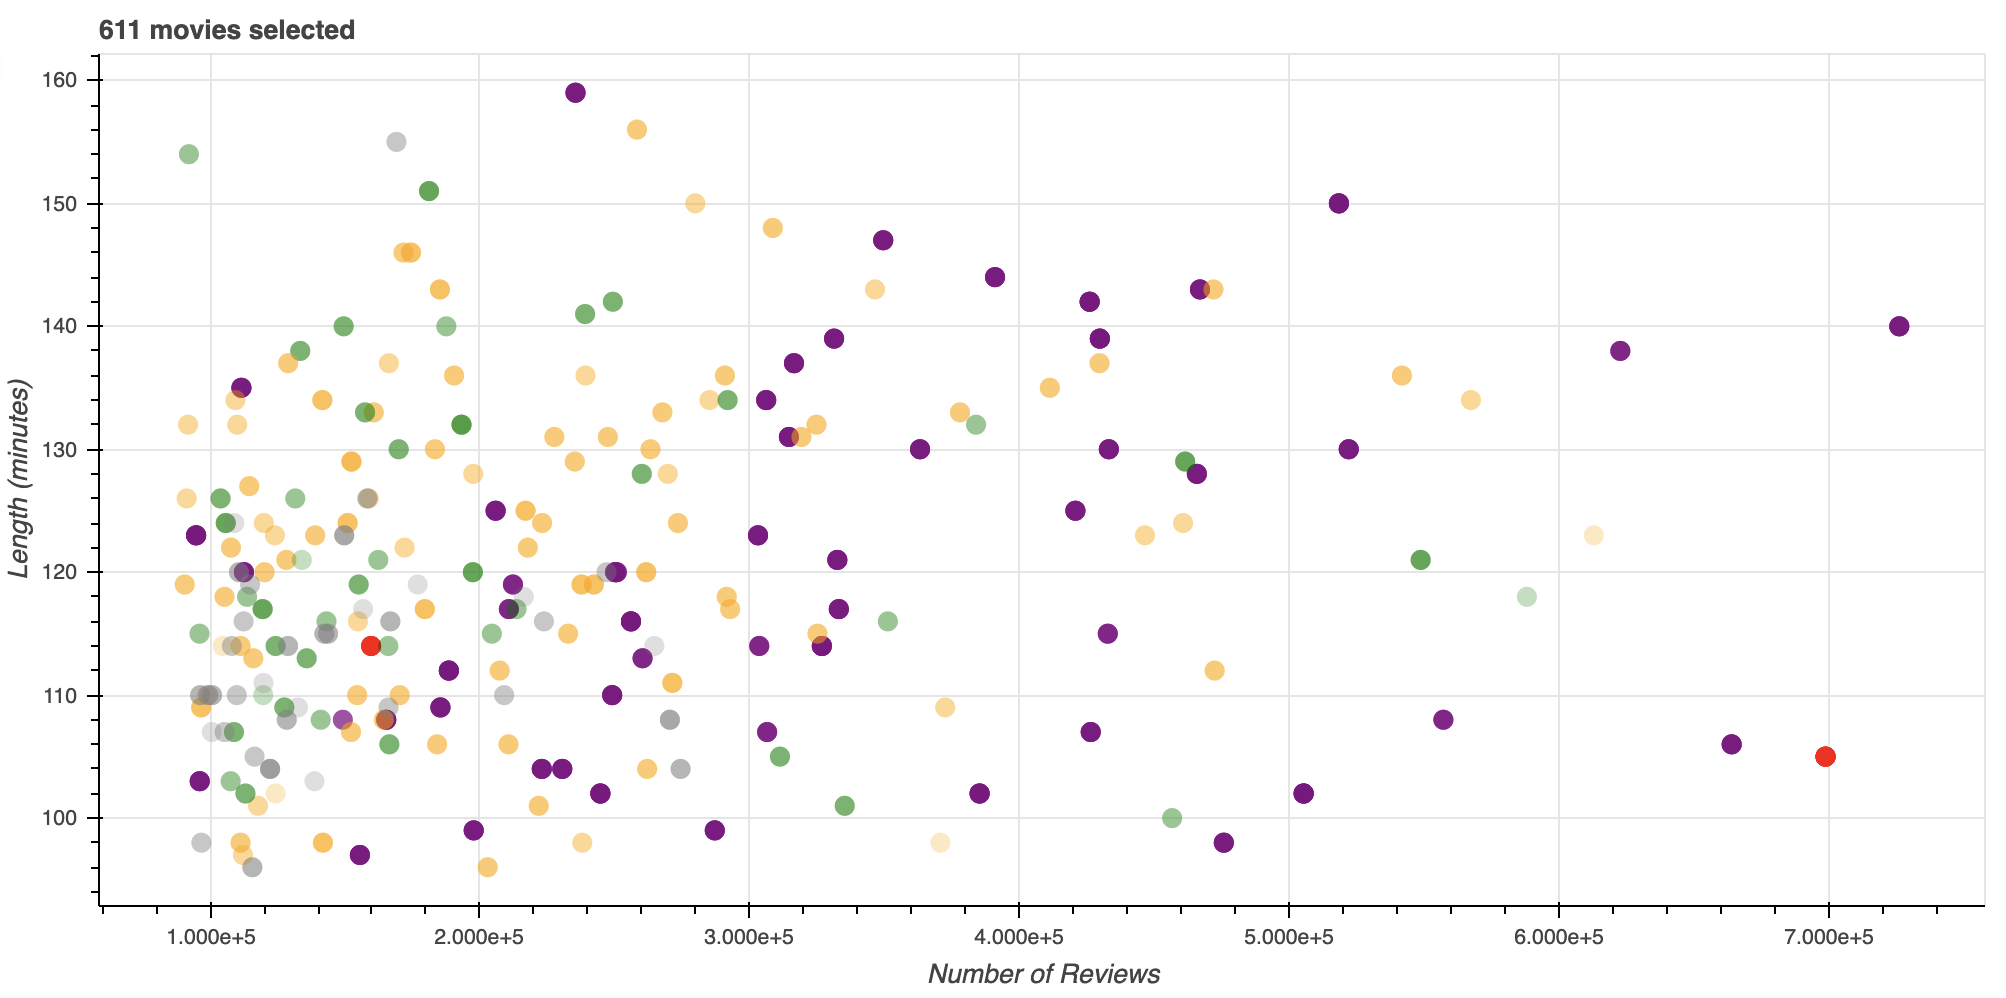
\includegraphics[width=300pt]{figures/review_length.png}
  \caption{Diagram of the review number and length of movie}
  \label{fig:review_length}
\end{figure}

\section{Data Analysis}
Here we firstly create some views to simplify the subsequent querying. These views temporarily store matches which we find between movies and their related entities. Listing~\ref{lst:query1} shows the creation of this view.
% FIXME

% FIXME
With those views, we could dig deep to find tendencies or some correlations in movie fields in decades. Figure~\ref{fig:rank}  shows the rank of a ratio where ratio equals to
\[
 \frac{\text{number of actors whose average rating exceeds 7.25 in one specific country}}{\text{number of actors in this country}}
\]

This rank of ratio reveals the different countries' movies' influence. The queries is shown in Listing~\ref{lst:query2}.
 In this ranking, we could find those countries which are not abundant in the movie industry obtain relatively high rankings because only their famous actors and movies are recorded in open source databases. The reason China gets a relatively low ranking is that China is a brand new movie market. Considering that quality always fails to catch up with quantity, this ranking is quite reasonable and indicates that there is still a long distance to develop for Chinese movies. \par

\begin{figure}[H]
  \centering
  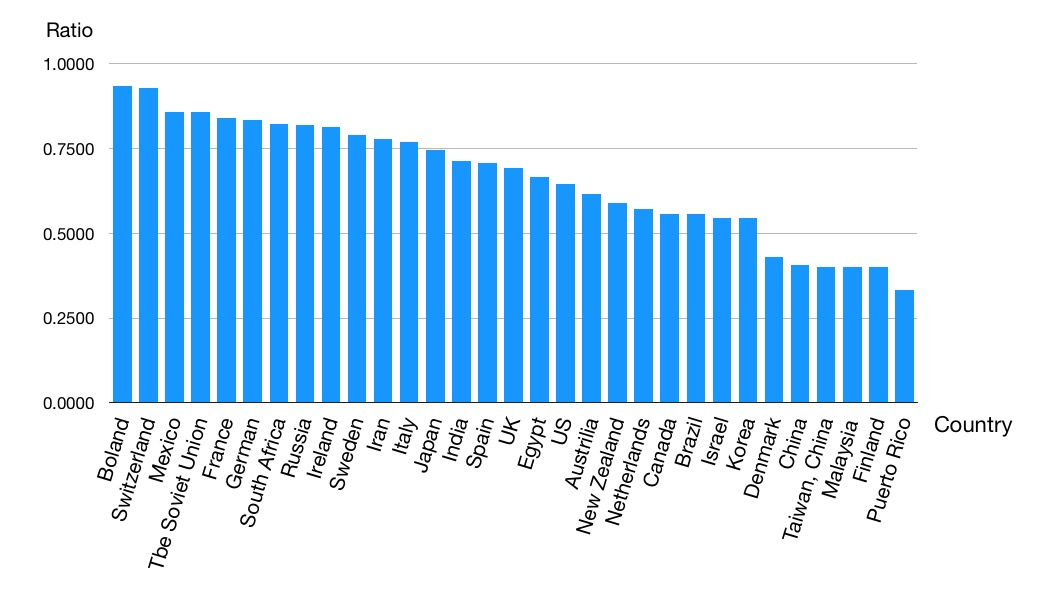
\includegraphics[width=320pt]{figures/rank.jpeg}
  % FIXME
  \caption{Rank of country about ratio of actors/actresses whose average rating grades exceed 7.25}
  \label{fig:rank}
\end{figure}
The Figure~\ref{fig:annual} could confirm the booming movie market. After counting the annual number and rating of movies, the tendency of the movie industry is evident. The barriers are falling for small firms. The amount of film increases rapidly, but the quality decreases step by step.

\begin{figure}[H]
  \centering
  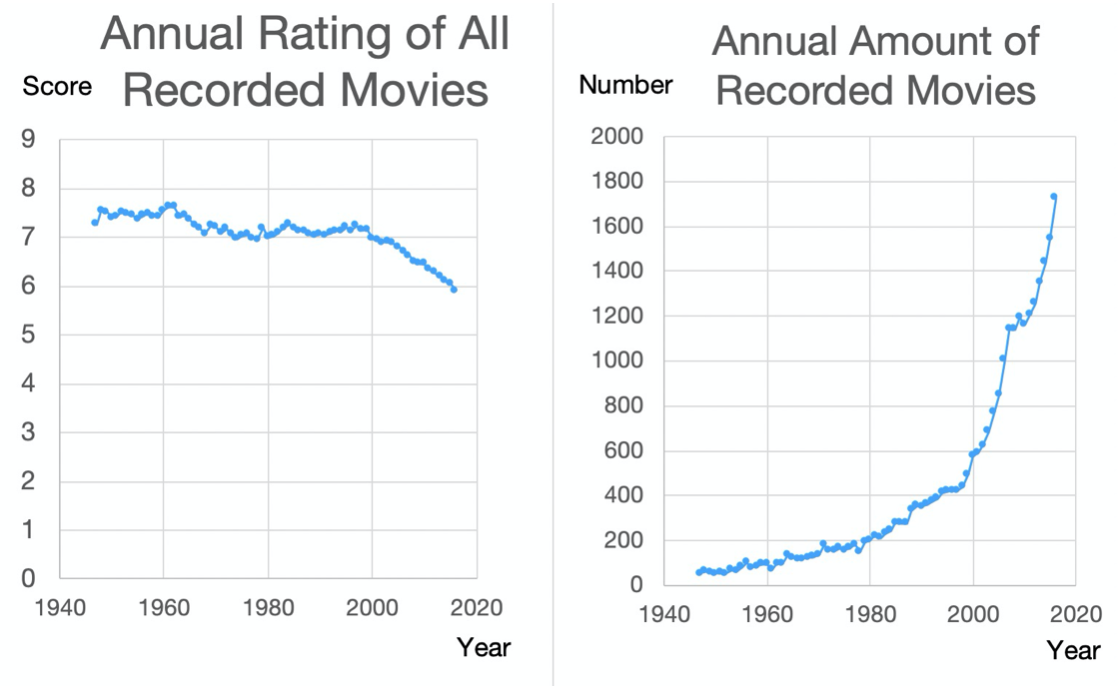
\includegraphics[width=250pt]{figures/annual.png}
  \caption{Annual rating of all recorded movies and annual amount of recorded movies}
  \label{fig:annual}
\end{figure}

\section{Self-evaluation}
  \subsection{What did we learn from the experience?}
  % \paragraph{What did we learn from the experience?}
  Since we realized the entire process of building a database system, we have learned and practiced many related objects, including:
  \begin{itemize}
    \item Analyze the requirements in a realistic situation.
    \item Identify and improve a database system design in Boyce-Codd normal form.
    \item Produce E-R diagram based on our database design.
    \item Data collection with web crawlers.
    \item Produce SQL queries for practical operations.
    \item Data analysis based on our database.
    \item Implement a visual website to demonstrate the database.
  \end{itemize}
  \subsection{What difficulties have we solved?}
    In this process, we also encountered some difficulties. Since the data is from several sources, therefore, part of the movies has been assigned different IDs in the different datasets. We need to match and link the same movie from the different datasets based on their attributes. Justifying our database designs are in good normalized form is also a challenge. To optimize our design, we make full use of the knowledge learned in the course and achieve a good result.

\section{Conclusion and Future Work}
In conclusion, we build an Enhanced Movie Database as an valuable source for aggregating movie reviews, searching, rating, and research. There is a large amount of realistic data in our database, which all come from several professional movie data websites, such as Douban and China Movie Data Information Network. The database is in a high-quality design, which is in Boyce-Codd normal form. We also provide adequate SQL queries for specific searching and selection. We show the value of our database by these queries that would have required exploring multiple web pages to answer. Through our database system, the researchers become much simpler to implement more comprehensive analysis and data mining. \par
For future work, there are other unused data, such as movie release type, producer company, and other multi-value attributes. Adding new entities and relationships can help enrich our database. Besides, because the size of our database is large, we will continue to work on improving the IO efficiency of our system for better user experience. On the other hand, although we provide some cases above, we are confident that researchers could utilize our project for more widely and more deeply  application of meaningful machine learning and social analytics. For instance, whether rating and box office of a movie is related to the number of actresses in that movie. We can also cluster all kinds of attributes of movies to find the common characteristics of high-quality/low-quality movies. These both can be engaging research topics. Therefore, using our database to conduct a profound study on movies may be an interesting way to explore.
\newpage

\bibliography{report}
\bibliographystyle{IEEEtran}
\newpage
\textbf{\section*{Appendices}}
\subsection*{SQL Queries}

\begin{lstlisting}[
caption={Pre-created Views Of Quick Querying},
captionpos=b,
language=SQL,
showspaces=false,
basicstyle=\ttfamily,
commentstyle=\color{blue},
label={lst:query1}
]
-- Movie, Actor, Rating
CREATE VIEW movie_actor_rating AS
SELECT movie_basic_info.Mid, title, rating, Aid, profession
FROM movie_basic_info, Actors_Movie
WHERE movie_basic_info.Mid = Actors_Movie.Mid
\end{lstlisting}

\begin{lstlisting}[
caption={SQL Queries of Figure~\ref{fig:rank}},
captionpos=b,
language=SQL,
showspaces=false,
basicstyle=\ttfamily,
commentstyle=\color{blue},
label={lst:query2}
]
CREATE VIEW country_725actor AS
SELECT COUNT(Actors_info.Aid), Country
FROM movie_actor_rating, Actors_info
WHERE movie_actor_rating.Aid = Actors_info.Aid AND profession = "Actor"
AND rating > 7.25
GROUP BY Country;

CREATE VIEW country_0actor AS
SELECT COUNT(Actors_info.Aid), Country
FROM movie_actor_rating, Actors_info
WHERE movie_actor_rating.Aid = Actors_info.Aid AND profession = "Actor"
GROUP BY E_name, C_name, Country;

SELECT number725_Actors/number0_Actors,country_725actor.country
FROM country_725actor, country_0actor
WHERE country_0actor.country = country_725actor.country
\end{lstlisting}

\subsection*{Labor Distribution}
\begin{itemize}
  \item Liu Yihan (117010007): Web crawler \& Design and normalization of E-R diagram and schema
  \item Cai Haoming (117010002): Web crawler \& Raw data preprocessing \& Data mining and analysis \& PPT Creating
  \item Huang Zihao (117010103): Raw data preprocessing \& Primary design and normalization of E-R Diagram and schema
  \item Chen Haoyu (117010013): Participation in the design of E-R diagram and normalization \& Data processing
  \item Cao Yuji (117010007): Web visualization implementation \& Primary design and normalization of E-R diagram \& Database building \& Report formatting

\end{itemize}

\subsection*{Source Code}

Our project structure is demonstrated in Figure~\ref{fig:file} as a tree diagram. ``database.db'' is our database with Sqlite database extension. ``src'' is the folder containing our source codes. Commands to run the web visualization application is listed in Listing~\ref{lst:web} and commands to view our database is listed in Listing~\ref{lst:sqlite}.
\begin{lstlisting}[
language=bash,
caption={Commands to run web visualization application},
morekeywords={pip, bokeh},
label={lst:web}
]
#!/bin/bash
pwd # ensure your current directory is in our project
pip install Bokeh # install Bokeh Python Library if there isn't
cd src/Web_Visualization
bokeh serve --show . # run the application
\end{lstlisting}

\begin{lstlisting}[
language=bash,
caption={Commands to view the database in terminal},
morekeywords={sqlite3},
label={lst:sqlite}
]
#!/bin/bash
pwd # ensure your current directory is in our project
sqlite3 database/movies.db
\end{lstlisting}

\begin{figure}[H]
  \centering
  \framebox[200pt]{%
    \begin{minipage}{180pt}
\dirtree{%
.1 project.
.2 report.pdf.
.2 database.
.3 movies.db.
.2 src.
.3 Analysis.
.4 query.sql.
.4 preprocess.py.
.3 Web\_Crawler.
.4 Actors.py.
.4 Awards.py.
.3 Web\_Visualization.
.4 Tabs.
.5 explorer\_tab.py.
.5 table\_tab.py.
.4 description.html.
.4 explorer.sql.
.4 genres.txt.
.4 main.py.
.3 data\_processing.
.4 actor\_award.py.
.4 actor\_movie.py.
.4 comm\_users.py.
.4 movies.py.
.4 user.py.
}
    \end{minipage}
}
\caption{Project Structure}
\label{fig:file}
\end{figure}

\end{document}
